% Chapter Template

\chapter{La piattaforma ARM embedded} % Main chapter title

\label{Chapter5} % Change X to a consecutive number; for referencing this chapter elsewhere, use \ref{ChapterX}

\lhead{Capitolo 5. \emph{La piattaforma ARM embedded}} % Change X to a consecutive number; this is for the header on each page - perhaps a shortened title

%-------------------------------------------------------------------------------
%	SECTION 1
%-------------------------------------------------------------------------------

\section{Sistema \emph{embedded}}

%Sistema embedded: che cos'è, a che cosa serve, chi rientra nella categoria?
%Differenza tra special purpose e general purpose, importanza dell'applicazione
// Rivedere questo incipit \\
Un sistema può essere visto come un insieme di più parti che collaborano al fine
di svolgere un determinato compito; considerando gli  ambiti informatici ed 
elettronici un sistema \emph{embedded} (tradotto solitamente con ``sistema 
integrato'')
 \\ \\
// Aggiungere parti al paragrafo precedente in modo da connetterlo al prossimo
 \\ \\
Un \emph{personal computer} deve saper rispondere a necessità disomogenee: 
lo stesso PC potrebbe essere acquistato da alcuni per essere utilizzato come 
\emph{word processor}, da altri come riproduttore multimediale, e da svariate 
ulteriori persone con diversi scopi. Questo rende indispensabile la 
realizzazione di un sistema \emph{general purpose}, ovvero un sistema che possa 
essere riconfigurato velocemente (ad esempio installando del software 
specifico) a seconda della funzione che bisogna svolgere in quel momento.
Un sistema \emph{embedded}, invece, è caratterizzato dall'essere un dispositivo 
\emph{special purpose}, ovvero dal dover svolgere un'unica funzione (i.e., 
avere un'unica applicazione) impiegando tutte le risorse disponibili.
Un sistema di questo tipo è ad esempio una centralina di un'automobile: il 
microcontrollore che svolge questo compito deve impiegare tutte le sue risorse 
(memoria, CPU, interfacce I/O) per elaborare i dati che riceve dai sensori e 
agire in conseguenza di determinate evenienze (e.g., se le ruote slittano 
allora attiva l'ABS). Il sistema in questione sarà programmato in modo da 
svolgere al massimo delle sue capacità queste funzioni, diventando un elemento 
\emph{specializzato} nel suo compito, privo di qualsiasi flessibilità presente 
in un dispositivo \emph{general purpose}.
\\ // Aggiungere paragrafo di collegamento al paragrafo successivo \\
La specializzazione non è sicuramente l'unico motivo per cui un sistema 
\emph{embedded} ottiene \emph{performance} migliori rispetto ad un generico PC; 
considerando anche solamente l'unità d'elaborazione, la CPU del primo possiede 
una frequenza ed un numero di transistor minore (mediamente di un fattore 10) 
rispetto alla CPU del secondo. Un discorso simile può essere intrapreso con la 
velocità della memoria volatile.
Alcuni tra gli ulteriori  motivi per preferire un sistema integrato sono:
\begin{itemize}
\item Presenza di architettura di memoria Harvard
\item \emph{CPU design} basato su RISC anziché CISC\footnote{Reduced 
Instruction Set Computing e Complex Instruction Set Computing}
\item Presenza di funzioni \emph{intrinsic} specifiche per le applicazioni più 
comuni
\item Presenza di hardware dedicato
\end{itemize}
// Inserire motivazioni dei punti in lista \\
Ma le pure prestazioni non sono l'unico motivo per cui preferire un sistema 
\emph{embedded}, tra gli altri presupposti possiamo includere:
\begin{itemize}
\item Consumi estremamente ridotti
\item Costi contenuti
\item Durata commerciale molto estesa
\end{itemize}
// Inserire motivazioni dei punti in lista
%-------------------------------------------------------------------------------
%	SECTION 2
%-------------------------------------------------------------------------------

\section{Processori ARM}

%-----------------------------------
%       SUBSECTION 1
%-----------------------------------

\subsection{Il processore AllWinner A20}

%-------------------------------------------------------------------------------
%       SECTION 3
%-------------------------------------------------------------------------------
\newpage
\section{Il \emph{single-board} computer Banana Pi M1}
\begin{center}
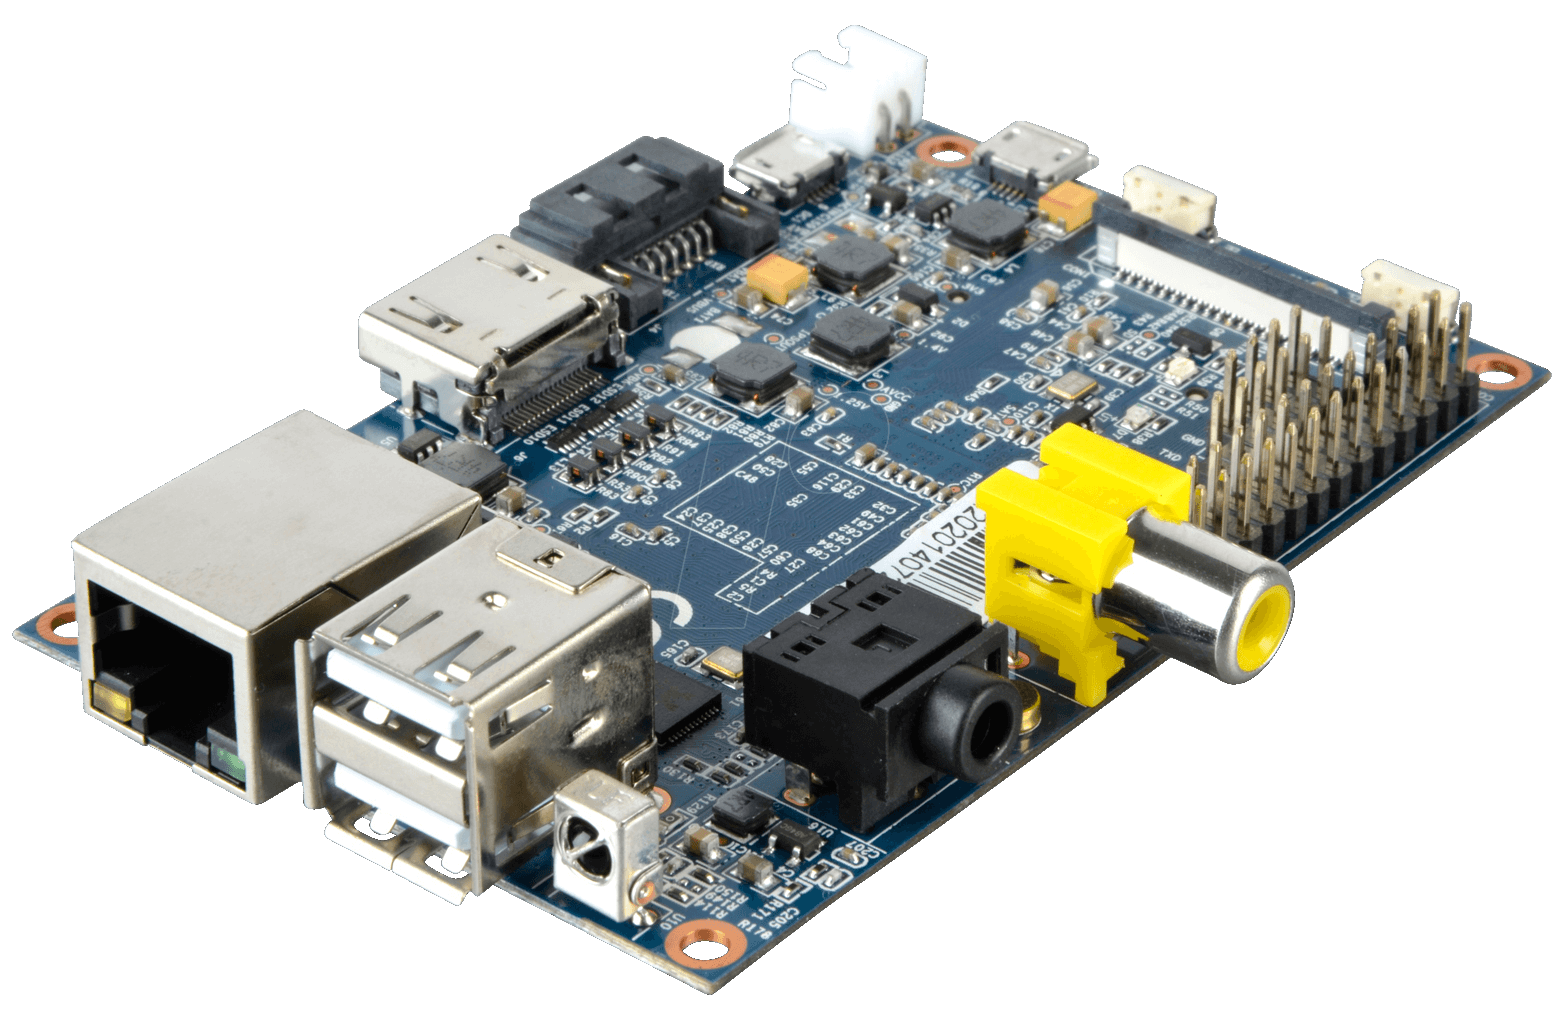
\includegraphics[scale=0.175]{Figures/bananapi.png}\\
\end{center}
Il termine \emph{single-board} viene usato per indicare un'implementazione 
circuitale che sia a tutti gli effetti un computer pur non presentando il 
classico schema con \emph{motherboard, daughterboard} e CPU separate in diverse 
schede: un solo circuito stampato contiene tutte e tre. 
